\chapter{\glsentrytext{Privacy} در \glsentryplural{CachingSystem}}
\label{chap:privacyInCaching}

\begin{abstract}

افزایش روزافزون 
\glspl{MultimediaApplication}،
موجب رشد ‌فزاینده‌ی ترافیک در شبکه‌های کنونی گشته است. انتقال این حجم عظیم از داده در ساعات اوج مصرف، همواره یکی از چالش‌های بزرگ طراحان شبکه بوده است؛ چراکه در این حالت، بسیاری از 
\glspl{Link}ی
شبکه به مرز اشباع خود می‌رسند، که این خود موجب افزایش چشمگیر
\gls{Delay}
و کاهش
\gls{QoE} \glspl{User}
می‌گردد. استفاده از
\glspl{NetworkCachingSystem}،
یکی از روش‌های موثر برای حل این معضل محسوب می‌گردد
\cite{Borst2010Distributed}.

همان‌طور که در
\autoref{fig:deliverscenarios}
مشاهده می‌کنید، 
\gls{User}ی در \gls{Coverage} یک \gls{AP}
قرار گرفته است. \gls{AP} نیز  به
\gls{Server}
اصلی شبکه متصل است.  هدف غایی این شبکه، ارسال 
\gls{Content}ی
مورد نیاز 
\gls{User}
از \gls{Server} به اوست.  در
\glspl{NetworkCachingSystem}
در طول ساعات‌ کم‌ترافیک، مرحله
 \gls{Replacement}
 صورت می‌پذیرد. در طول این مرحله برخی از \glspl{Content}یی که \glspl{User} ممکن است در ساعات اوج ترافیک بدان نیاز داشته‌باشند، در 
\gls{Cache} \gls{AP}
قرار می‌گیرد. در ساعات اوج مصرف با رسیدن درخواست
 \gls{User}،
 ابتدا \gls{AP} چک می‌کند که
\gls{Content}ی
مورد نظر در \gls{Cache} وجود دارد یا نه؟ در صورت وجود، \gls{AP} بدون رهسپار نمودن درخواست به \gls{Server}  اصلی، خود به سرعت 
\gls{Content}ی
موردنظر را  برای \gls{User} ارسال می‌کند. در غیر این صورت \gls{AP} درخواست  \gls{User} را به \gls{Server}‌ا صلی می‌دهد. به این مرحله که عموما در ساعات اوج ترافیک صورت می‌پذیرد، اصطلاحا مرحله
\gls{Delivery}
گفته می‌شود
\cite{MaddahAli2012Fundamental}.
این مرحله به خوبی در
\autoref{fig:deliverscenarios}
نشان داده شده است. 

 بیشتر کارهای تحقیقاتی موجود در حوزه
\glspl{CachingSystem}،
بر روی تعین
\gls{Policy} \gls{Optimal} برای نحوه پر کردن \glspl{Cache}, \gls{Capacity} این \gls{System} و \gls{Privacy} \gls{Content}ی
داده مبادله شده، تمرکز کرده‌اند
\cite{MaddahAli2012Fundamental,Niesen2014Coded,Sengupta2014Fundamental,Sengupta2014Decentralized}.
باتوجه به مطالعات صورت‌پذیرفته، تاکنون کاری در مورد حفظ
\gls{Privacy} \gls{ContextOriented} در \glspl{CachingSystem}
صورت نگرفته است. ما بر آنیم تا در این فصل بر روی این موضوع متمرکز شویم.

در 
\autoref{sec:motivatingExample}
نخست سعی داریم تا با یاری جستن از یک مثال ساده، خلا 
\gls{Privacy} \gls{ContextOriented}، در \glspl{CachingSystem}
را متذکر شویم. در
\autoref{sec:contributionCache}،
به تشریح نوآوری‌های بدست آمده، خواهیم پرداخت. 
\autoref{sec:systemModelCaching}
را به بیان 
\gls{SystemModel}
تخصیص می‌دهیم. روش پیشنهادی به همراه تحلیل ریاضیاتی آن در 
\autoref{sec:proposedanaCaching}
خواهد آمد. در نهایت نیز
\gls{Simulation} و \gls{NumericalAnalysis}
روش پیشنهادی، در
\autoref{sec:Simulation}
بیان خواهد شد. 




\begin{figure}
\begin{subfigure}[b]{0.7\textwidth}\centering
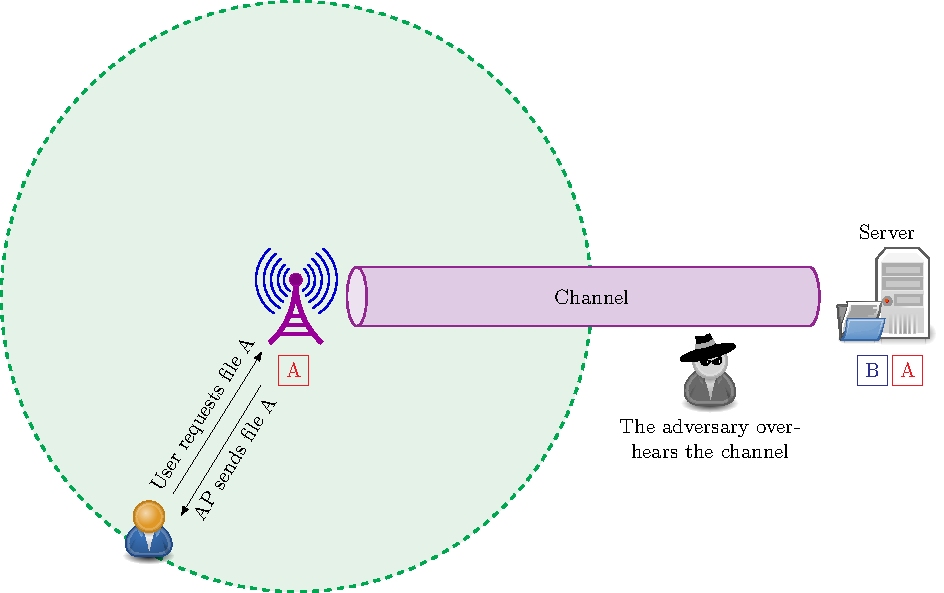
\includegraphics[width=\linewidth]{Pic/cachingSystemTotal/mainFig}
\caption{}
\label{fig:cachingSystemTotal1}
\end{subfigure}\\*[10mm]
\begin{subfigure}[b]{0.7\textwidth}\centering
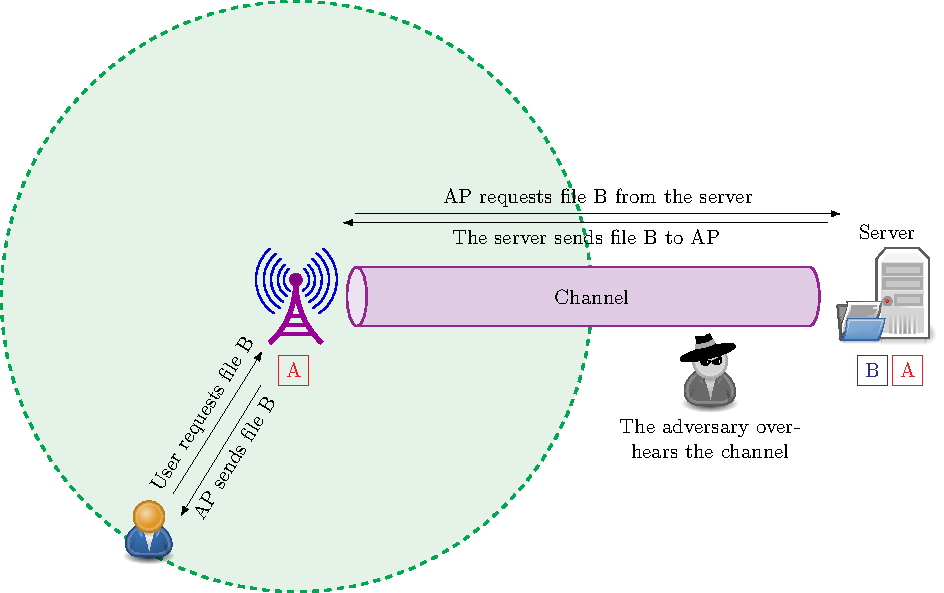
\includegraphics[width=\linewidth]{Pic/cachingSystemTotal/mainFig2}
\caption{}
\label{fig:cachingSystemTotal2}
\end{subfigure}
\caption{\lofimage{Pic/cachingSystemTotal/mainFig}
(آ)
\glsentrytext{User}
از 
\glsentryname{AP}
درخواست فایل \lr{A} را می‌کند. چون
\glsentryname{AP} در \glsentrytext{Cache}
خود این فایل را دارد، بدون درخواست از
\glsentrytext{Server}
اصلی، این فایل را به
\glsentrytext{User}
در مدت زمانی اندک ارسال می‌کند. (ب)
\glsentrytext{User}
از 
\glsentryname{AP}
درخواست فایل \lr{B} را می‌کند. چون
\glsentryname{AP} در \glsentrytext{Cache}
خود این فایل را ندارد، مجبور است  از
\glsentrytext{Server}
اصلی بخواهد که این فایل را برای او ارسال کند. با دریافت این فایل توسط 
\glsentryname{AP}
 او آن را به 
\glsentrytext{User}
می‌دهد.}
\label{fig:deliverscenarios}
\end{figure}


\end{abstract}

\section{مثال انگیزه‌بخش}
\label{sec:motivatingExample}


\section{نوآوری‌ها}
\label{sec:contributionCache}


\section{\glsentrytext{SystemModel}}
\label{sec:systemModelCaching}


\section{روش پیشنهادی}
\label{sec:proposedanaCaching}

\section{\glsentrytext{Simulation} و \glsentrytext{NumericalAnalysis}}
\label{sec:Simulation}



